	En este capítulo definimos el problema que deseamos atacar. Éste se encuentra específicamente identificado en las escuelas de nivel superior del Instituto Politécnico Nacional. \\
	Como problema general encontramos que la comunicación entre sectores (alumnos, profesores y personal administrativo) no cuenta con un medio masivo para simplificar la interacción entre ellos y dificulta el traslado de la información hacia su destinatario.\\
	El problema general podría ser desglosado en una gran cantidad de problemáticas particulares, este trabajo se centrará en las siguientes aquí descritas.
	\section{Problemáticas Identificadas}
	
		La comunicación dentro de la comunidad estudiantil de la Escuela Superior de Cómputo (ESCOM) es un tema de controversia. Actualmente existen problemas para lograr la correcta conexión entre los alumnos y profesores, de la misma manera con muchas de las áreas que tiene la institución. Esto no es un problema propio de alguna de las partes, son una serie de circunstancias que obstaculizan la correcta comunicación entre los sectores de la comunidad. Entre otras cosas, afecta la falta de interés por acercarse a las dependencias de la escuela para obtener informes así como lo confusa que es la difusión de los diversos trámites que se ofrecen y lo dispersa que esa información está, ya que cada departamento cuenta con sus medios para difundirla.\\
	
	La problemática antes descrita afecta a la comunidad estudiantil y el trabajo se enfoca en los siguientes puntos:
	\begin{itemize}
		\item \textbf{\textit{Dificultad para localizar las áreas o espacios de la Escuela Superior de Computo.}}\\
		
		Este es uno de los principales problemas a atacar. Entendemos que en muchas ocasiones es complicado identificar las distintas áreas con las que cuenta la Escuela. Hay oficinas de dirección en distintos edificios, así como los departamentos que gestionan diversos trámites, etc. Esto no solo afecta a los alumnos de nuevo ingreso y personas visitantes, sino también a alumnos de semestres más avanzados que no terminan por ubicar las áreas que necesiten en el momento. Por ejemplo muchos no conocen la ubicación de las áreas de la ESCOM, tales como: Dirección, Subdirección Académica, Coordinación de Desarrollo Tecnológico, Recursos Materiales, Decanato, etc.\\ 
		
		
		La forma más sencilla de identificar un espacio es mediante su nomenclatura.
		
		Los salones tienen dos nomenclaturas. Definida para los salones de la siguiente manera:
		\begin{itemize}
			\item Número de edificio
			\item Número de piso
			\item Número de salón
		\end{itemize}
		
		Tomando el salón \textbf{2201} como ejemplo:
		
		El primer \textbf{2} de izquierda a derecha es el número de edificio de la institución, el segundo \textbf{2} es el piso del edificio y finalmente el \textbf{01} es el número del salón.\\
		
		\begin{itemize}
			\item Número de salón
			\item Letra 'N' para "Norte"  y  'S' para "Sur" de acuerdo a  la ubicación del salón
		\end{itemize}
		
		Tomando la sala \textbf{21N} como otro ejemplo: 
		
		El número \textbf{21} indica el número de salón y \textbf{N} que indica que el salón esta orientado hacia el Norte\\
		
		En la entrada principal de la Escuela Superior de Cómputo existe un mapa de localización de las áreas de la escuela el cual no contempla todas las existentes.  Lo que nos genera problemas de comunicación entre la institución y las personas que están en ellas. \\ 
		
		 Durante la primera semana de inicio de semestre, el mayor problema que se presenta es la forma en la que se difunde la asignación de salones donde se impartirán las clases, lo que implica perdida de tiempo al buscar la ubicación del salón asignado, perdida de tiempo al buscar la pancarta impresa de la asignación de los salones, desencadenando en la posibilidad de no llegar puntuales a las primeras clases. En la figura \ref{fig:graficacubiculos}, \ref{fig:graficadepartamentos} y \ref{fig:graficadesalones} se pueden ver los resultados de una encuesta realizar a los estudiantes de la Escuela Superior de Cómputo\\ \\
		\begin{figure}[ht]
			\centering
			\caption{Ubicaci{\'o}n de Cub{\'i}culos}
			\label{fig:graficacubiculos}
			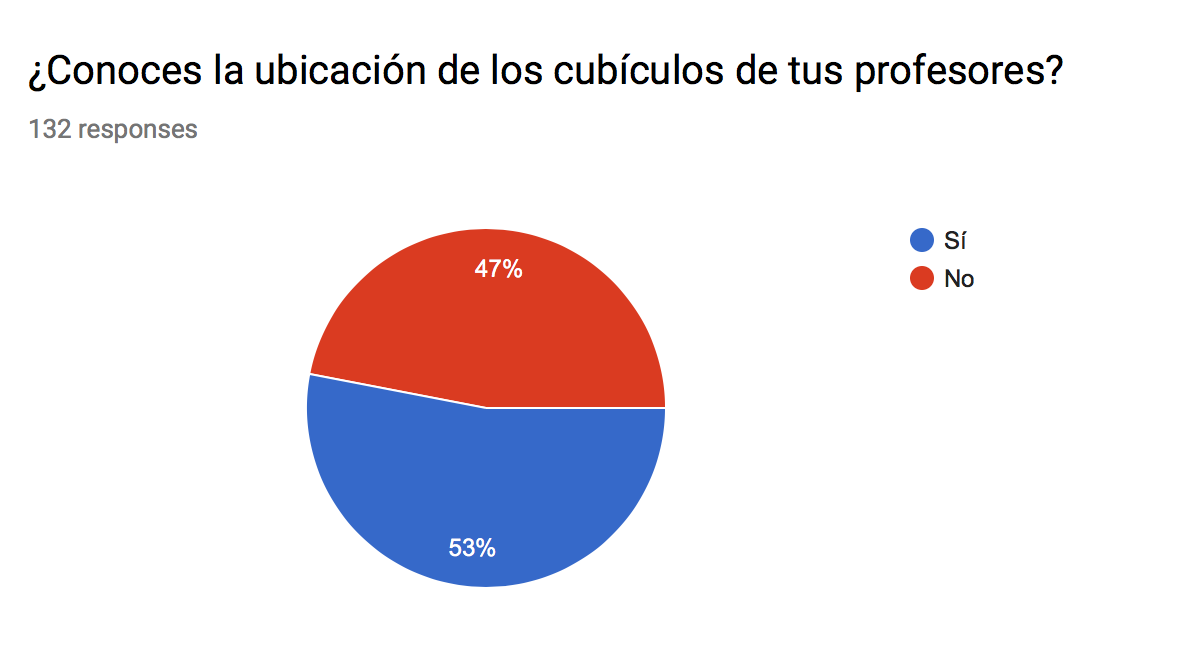
\includegraphics[width=.5\textwidth]{PlanteamientoProblema/cubiculos}
		\end{figure}
	
	\begin{figure}[ht]
		\centering
		\caption{Ubicaci{\'o}n de departamentos}
		\label{fig:graficadepartamentos}
		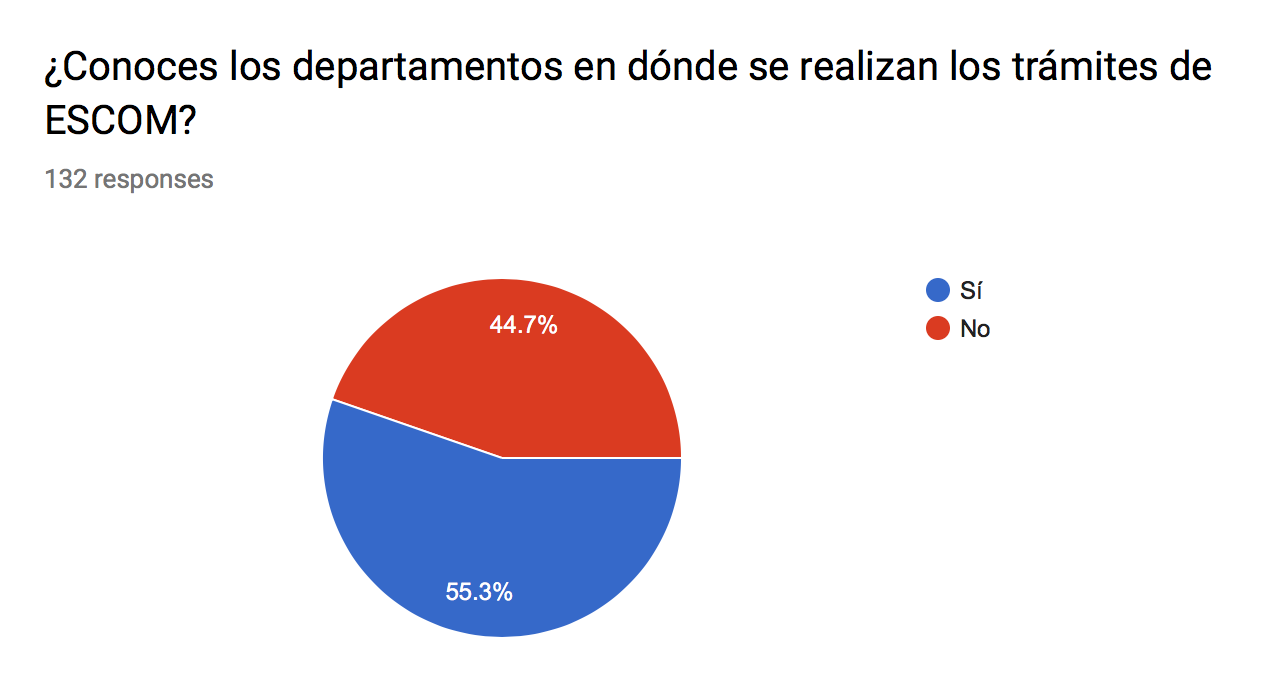
\includegraphics[width=.5\textwidth]{PlanteamientoProblema/departamentos}
	\end{figure}

	\begin{figure}[ht]
	\centering
	\caption{Consulta de salones}
	\label{fig:graficadesalones}
	
\includegraphics[width=.5\textwidth]{PlanteamientoProblema/salones}
\end{figure}

		\item \textbf{\textit{Complicaciones al obtener material de apoyo.}} \\
		
		Si bien es cierto, el ser autodidacta es uno de los puntos mas importantes que debe tener un estudiante de la ESCOM para poder complementar su desarrollo académico, el  acceso al material educativo fuera de la escuela es complicado, ya que existen pocos elementos extracurriculares.\\
		
		Dentro de la institución se maneja una herramienta llamada Moodle, la cuál es una aplicación dirigida a la educación que ayuda a contrarrestar este tipo de necesidades, sin embargo, esta está dirigida solo a los alumnos cuyos profesores tengan acceso y hagan uso a esta herramienta. La cuál usualmente es utilizada como plataforma de entregas o evaluaciones de actividades dejando lejos el material educativo para que los alumnos puedan aclarar o practicar los temas vistos en clase. \\
		
		La ayuda de un elemento que auxilie a los alumnos a obtener material de apoyo para repasar los temas vistos en clase, beneficiaría a los mismos facilitando la etapa de evaluaciones que se llevan a cabo a lo largo del semestre escolar.\\ \\
		
		\item \textbf{\textit{Dificultad en la  difusión de cursos y certificaciones gratuitas para los alumnos de la ESCOM y desaprovechamiento de los mismos.}}\\
		
		La Escuela Superior de Cómputo oferta una gran variedad de cursos y certificaciones para sus alumnos, éstas pueden ser tanto gratuitas como con algún costo no significativo. Sin embargo son desaprovechadas por un gran sector de la comunidad debido a que en ocasiones la difusión de estos cursos no tiene el alcance esperado. Esto resulta en un gran desperdicio de oportunidades de crecimiento académico para los alumnos.\\
		
		Los cursos que se ofertan en la ESCOM en su mayor parte son difundidos dentro de la escuela mediante ferias, folletos o carteles, entre otras formas. Consideramos que en la actualidad, los alumnos nos vemos menos identificados con este tipo de propagandas y dedicamos nuestra atención mayormente a medios digitales o móviles.
		
		Una solución propuesta es agregar otro tipo de difusión para que la comunidad esté informada de los recursos extracurriculares que ofrece la ESCOM. El poder visualizar desde tu dispositivo móvil todas aquellas certificaciones o cursos podrían llevar al alumnos a tomarlos, si estos cursos son de su interés. Teniendo la posibilidad de contar con una mejor cantidad de alumnos inscritos a este tipo de actividades.\\ 
		
		
		
		\item \textbf{\textit{Difusión confusa de los procesos relacionados con Movilidad Estudiantil.}}\\
		
		Este punto esta un poco relacionado con el anterior, puesto que en la ESCOM existe la posibilidad para los alumnos de dirigirse a otra universidad en calidad de movilidad estudiantil y vivir la experiencia de estudiar ya sea fuera de la ciudad o en el extranjero. \\
		
		La falta de comunicación entre este proceso y los alumnos, genera controversia y confusiones con los mismos, ya que en ocasiones no saben las fechas de convocatoria ni los requisitos que se necesitan para aplicar una movilidad. Esta oportunidad tan grande que brinda tanto el IPN como la ESCOM es de suma importancia y se debe fomentar aún mas esta oportunidad para poder dar renombre de la calidad estudiantil del instituto y de los mexicanos.\\
		
		Es por eso que se propone que las aplicaciones móviles funcionen como medio de difusión de convocatorias y requisitos así como de los lugares en donde se puede realizar la movilidad y así darle esa gran oportunidad a los alumnos de aprender de otras culturas y de como es realizar una vida en el extranjero.\\
		
	\end{itemize}
	
	\subsection{Propuesta de Solución}
	
	Es por eso que en este Trabajo Terminal se propone una aplicación móvil para ayudar al buen flujo de información y a la buena comunicación con la comunidad de la Escuela Superior de Cómputo para facilitar la vida académica de los alumnos y ayudar a resolver los problemas mencionados anteriormente.\\
	
	Con base en las necesidades de la comunidad estudiantil se pretende crear una aplicación móvil que contemple principalmente las siguientes características:
	\begin{itemize}
		\item Consulta de espacios dentro de la escuela.
		\item Consulta de los medios de contacto del personal docente.
		\item Consulta del listado de asignaturas impartidas durante el semestre.
		\item Noticias Académicas.
		\item  Consulta de material de apoyo.
	\end{itemize}
